\documentclass{article}
\usepackage{lastpage}
\usepackage[polish]{babel}
\usepackage[T1]{fontenc}
\usepackage[utf8]{inputenc}
\usepackage{graphicx}
\usepackage{fancyhdr}
\usepackage{xstring}
\usepackage{xcolor}
\usepackage{indentfirst}
\usepackage[none]{hyphenat}
\usepackage{subfig}
\usepackage{float}

\newcommand{\version}{v1.0.4}
\newcommand{\lastPage}{13}
\newcommand{\tab}{\hspace{1cm}}
\newcommand{\justy}[1]{
\StrSubstitute{#1}{ }{ \hfill}

}


\pagestyle{fancy}
\setlength
\headheight{40pt}
\renewcommand{\footrulewidth}{0.4pt}
\fancyhf{}

\rhead{Dokumentacja projektu}
\lhead{
\includegraphics[width=5cm]{images/pp.jpg}\newline Wydział informatyki i telekomunikacji}

\lfoot{Politechnika Poznańska}
\cfoot{Page \thepage\space of\space \lastPage}
\rfoot{19.03.2020r.}

\begin{document}
\begin{titlepage}
		\begin{center}
			
						\LARGE
			Politechnika Poznańska
			
			\vspace{0.3cm}
			
			\large
			Wydział informatyki i telekomunikacji
			
			\vspace{3.0cm}
			\huge
			\textbf{Dokumentacja projektu}
			
			\vspace{0.5cm}
			
			\large
			Dokumentacja projektu z zajęć Telefonia IP
			
			\vspace{2.4cm}
			
			\LARGE
			\textbf{Autorzy:}
			
			\vspace{0.3cm}
			
			Adrian Golczak 136239
			adrian.e.golczak@student.put.poznan.pl
			
			\vspace{0.3cm}
			
			Marcin Kubiak 136267
			marcin.w.kubiak@student.put.poznan.pl
			
			\vfill
			
			\normalsize
			Wersja: \version
			
			\vspace{2cm}
			

			
			19.03.2020 r.
			
		\end{center}
\end{titlepage}
\tableofcontents
\newpage
	\section{Charakterystyka ogólna projektu}
	\tab Przedmiotem projektu pn. 'Opracowanie bezpiecznego systemu komunikacji głosowej w sieci IP (VoIP) wraz z jego implementacją' jest opracowanie aplikacji mobilnej wyposażonej w odpowiednie algorytmy umożliwiające bezpieczną rozmowę pomiędzy dwoma użytkownikami aplikacji. Główną koncepcją projektu jest stworzenie tzw. poczekalni, w której zalogowani użytkownicy bedą mogli się łączyć z kim tylko chcą i odbywać z nim rozmowę. Aplikacja będzie spełniała zasady integralności i poufności, aby uniemożliwić podsłuchanie rozmowy przez osobę trzecią.

	\section{Architektura systemu}
	\subsection{Uproszczona architektura technologii}
\tab Funkcjonalnie, możliwe będzie połączenie dwóch clientów aplikacji mobilnej poprzez server napisany w spring boot framework.\\
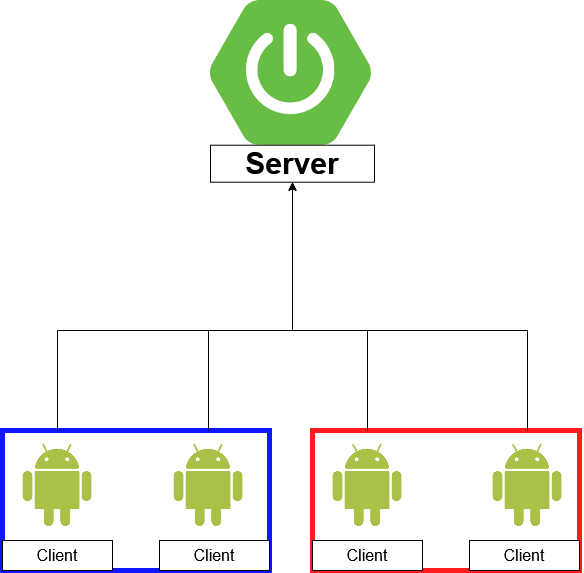
\includegraphics[width=12cm]{images/simple architecture.png}
\begin{center}
	\footnotesize
	Rysunek 1. Uproszczona architektura systemu
\end{center}
\subsection{Architektura przepływu}
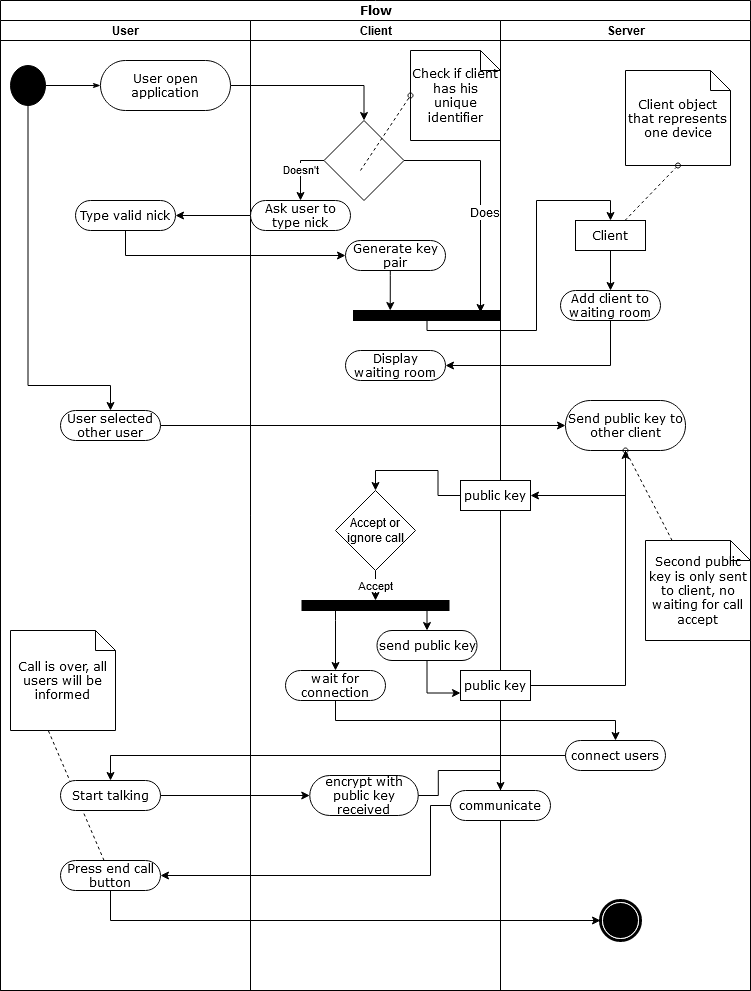
\includegraphics[width=12cm]{images/flow.png}
\begin{center}
	\footnotesize
	Rysunek 2. Architektura przepływu komunikacji pomiedzy użytkownikiem, klientem, a serwerem.
\end{center}
	\section{Wymagania}
	\justy{Poniżej opisane zostaną wymagania funkcjonalne i niefunkcjonalne aplikacji, z wyróżnieniem różnych stanów użytkownika.}
	\subsection{Funkcjonalne}
	\tab funkcjonalne
	\subsection{Niefunkcjonalne}
	\begin{itemize}
\item łączenie dwóch użytkowników,
\item generowanie ID sesji
\item negocjacje klucza o rozmiarze 256 bitów na potrzeby AES-256,
\item szyfrowanie rozmowy wykorzystując AES-256,
\item minimalna wersja systemu Android: 10.0.0,
\item brak wymogu podania hasła przez użytkownika przy logowaniu,
\item limit użytkowników w poczekalni podyktowany mocą obliczeniową serwera,
\item jedno urządzenie mobilne to jedna instancja klienta,	\item w ramach jednego pokoju może przebywać jedynie dwóch użytkowników,
\item zmiana głośności rozmowy za pomocą wbudowanych funckji sprzętowych urządzenia.
\end{itemize}

	\section{Technologie, narzędzia, środowisko, biblioteki, kodeki}
	\begin{itemize}
	\item \textit{TeXstudio}
	\item \textit{InteliJ}
	\item \textit{Java11}
	\item \textit{SpringBoot}
	\item \textit{AndroidStudio}
	\item \textit{javax.sound}
\end{itemize}
	\section{Ekrany}
	\justy{Poniżej zaprezentowano wstępne makiety ekranów jakie będą używane w aplikacji mobilnej, do obsługi dodawania użytkownika do kolejki, dzwonienia, odbierania połączeń, rozmowy i kończenia rozmowy. Wszystkie ekrany są jedynie koncepcją interfejsu i nie należy traktować ich jako produktu końcowego.}
\hfil


\begin{figure}[H]
	\centering
	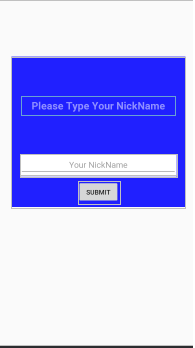
\includegraphics[width=8cm]{images/5.png}
	\caption{\centering Pierwszy ekran z prośbą o podanie pseudonimu użytkownika.}
	\hfill 
\end{figure} 
\begin{figure}[H]
	\centering
	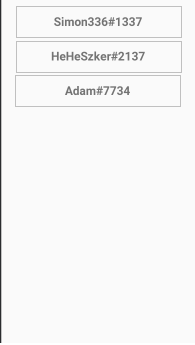
\includegraphics[width=8cm]{images/1.png}
	\caption{\centering Ekran z widoczną ''poczekalnią'', w której znajduje się trzech użytkowników.}
	\hfill 
\end{figure} 
\begin{figure}[H]
	\centering
	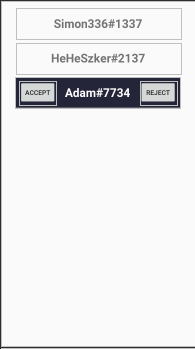
\includegraphics[width=8cm]{images/2.png}
	\caption{\centering Informacja o nadchodzącym połączenia od użytkownika Adam.}
	\hfill 
\end{figure} 
\begin{figure}[H]
	\centering
	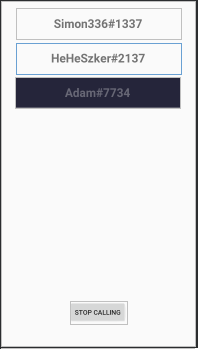
\includegraphics[width=8cm]{images/3.png}
	\caption{\centering Próba połączenia się z użytkownikiem Adam.}
	\hfill 
\end{figure} 
\begin{figure}[H]
	\centering
	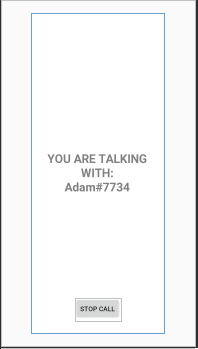
\includegraphics[width=8cm]{images/4.png}
	\caption{\centering Rozmowa z użytkownikiem Adam.}
	\hfill 
\end{figure}
\hfill

	\section{Diagramy UML}
	{W tym rozdziale skupimy się na 4 typach diagramów UML: przypadków użycia, przebiegów, stanów oraz klas.}
	\subsection{Diagram przypadków użycia}
	\vspace{0.5cm}
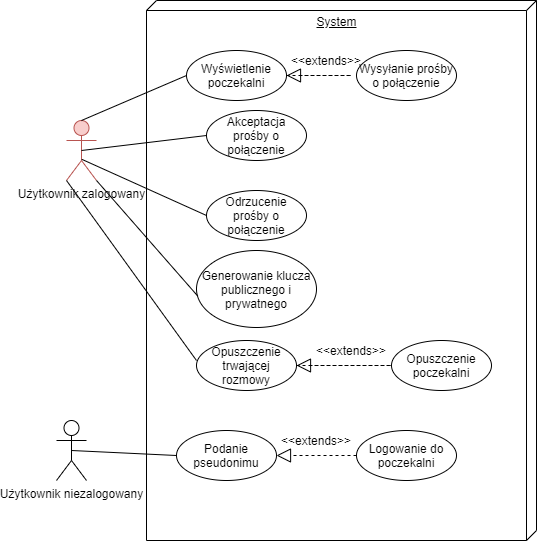
\includegraphics[width=\textwidth]{images/TIP-diagramPU.png}	
\caption{Rysunek 1: Diagram przypadków użycia z podziałem na dwóch aktórów: użytkownika zalogowanego i niezalogowanego}





	\subsection{Uproszczony diagram przepływu}
	\justy{Poniżej zaprezentowano uproszczony diagram przepływu. Diagram podzielono na 3 obiekty: użytkownika aplikacji, klienta, czyli aplikację mobilną będącą pośrednikiem pomiędzy użytkownikiem, a serwerem, i serwer który obsługuje wszystkie zapytania i odpowiednio je przetwarza, zarządza sesjami i połączeniami.}

\begin{figure}[H]
	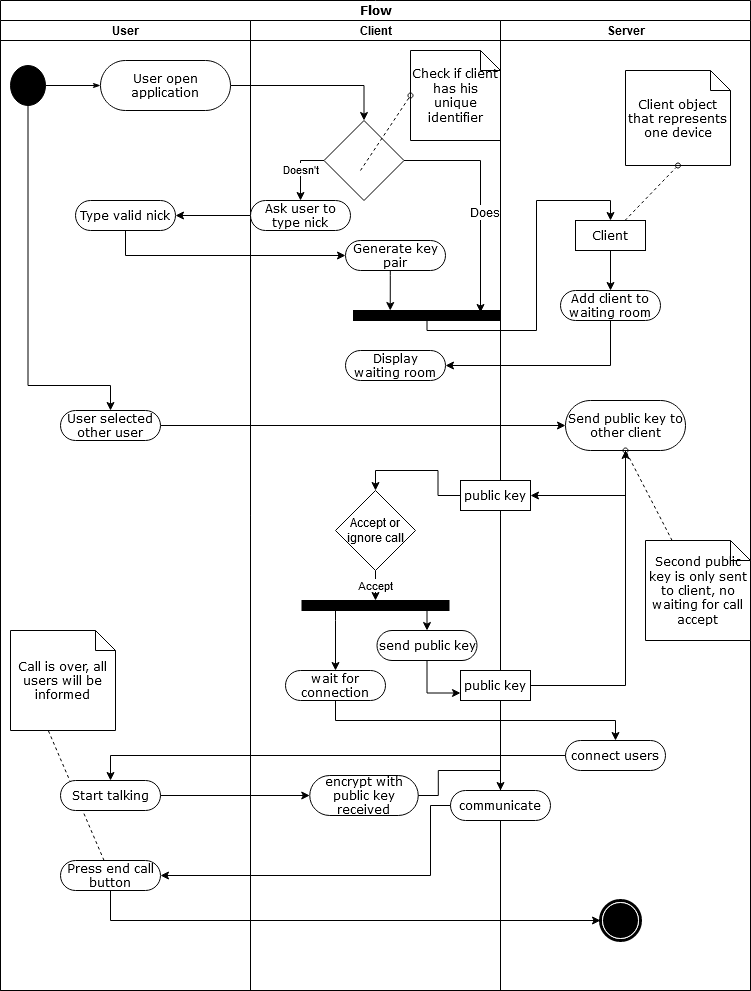
\includegraphics[width=\textwidth]{images/flow.png}
	\centering	
	\caption{\centering Uproszczony diagram przepływu przedstawiajacy inicjalizację sesji, a także dodania użytkownika do poczekalni.}
\end{figure}
	\section{Implementacja serwera}
	\justy{W tej sekcji prezentujemy najciekawsze fragmenty kodu aplikacji serwerowej. Jako wzorzec projektowy do wytwarzania oprogramowania użyliśmy Domain Driven Design, dzięki czemu podzieliliśmy kod na domeny, a to pozwoliło utrzymać go w ''czystości'' i ułatwia ewentualną późniejszą rozbudowę.}

\subsection{RegisterService}
\just{Serwis ten ma za zadanie zarządzać poczekalnią, dodawać i usuwać z niej użytkowników. Poczekalnia jest wstrzykniętą listą użytkowników przy użyciu Inversion of Controll Container'a, jako implementacji Dependency Injection.}

\begin{figure}[H]
	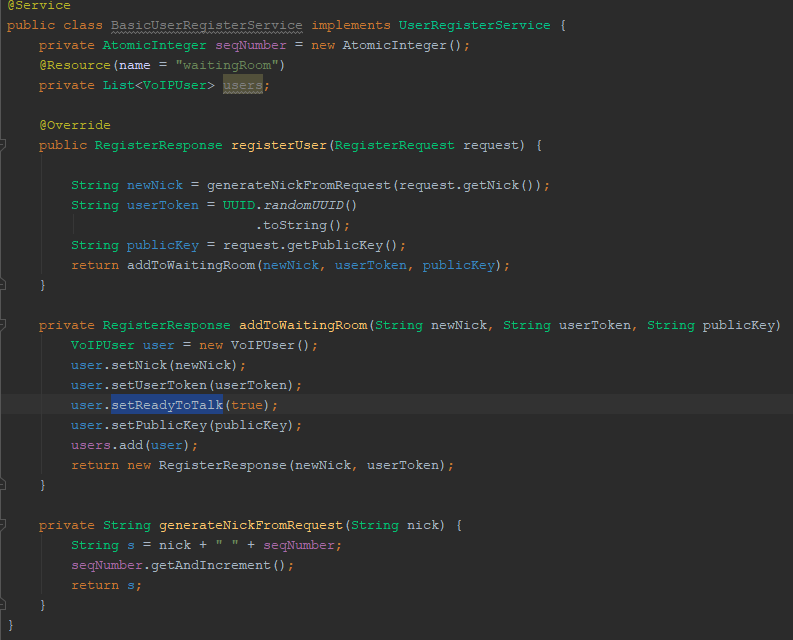
\includegraphics[width=\textwidth]{images/code1.png}
	\centering	
	\caption{\centering Kody serwisu zarządzającego użytkownikami i poczekalnią.}
\end{figure}

\subsection{ConnectionService}
\justy{Serwis odpowiedzialny za łączenie i rozłączanie użytkowników pośrednio wykorzystuje SessionService który zarządza dodatkowo sesjami użytkowników.}

\begin{figure}[H]
	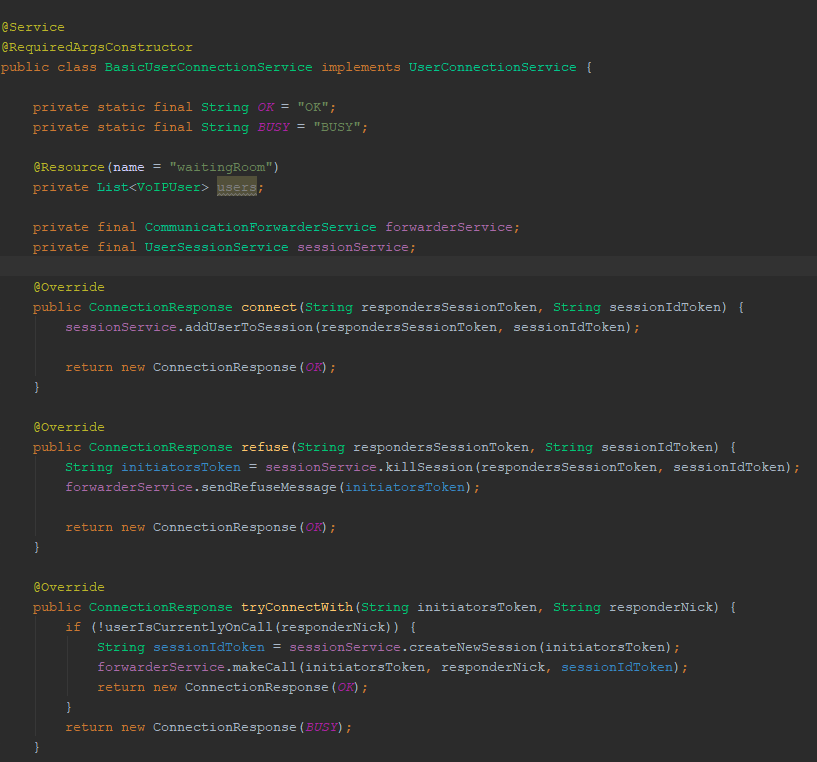
\includegraphics[width=\textwidth]{images/code2.png}
	\centering	
	\caption{\centering Klasa zarządzająca połączeniem użytkowników podczas próby rozmowy.}
\end{figure}
\end{document}
